\documentclass[11pt]{article}
%\usepackage[14pt]{extsizes} % для того чтобы задать нестандартный 14-ый размер шрифта
%\usepackage[utf8]{inputenc}
\usepackage{mathtext}
\usepackage[english, russian]{babel}
\usepackage{amsmath}
\usepackage{amsfonts}
\usepackage{float}
\usepackage[margin=0.8in]{geometry}
\usepackage{multirow}
\usepackage{graphicx}
\usepackage[utf8x]{inputenc} % указать кодировку русского текста
\usepackage{fancyhdr}
\usepackage{indentfirst} % отступ в первой строке абзаца
\usepackage{wrapfig}
\usepackage{placeins}
\usepackage{wrapfig}
\usepackage{caption}
\usepackage{amssymb}
\usepackage{mathtools}
\usepackage[thinc]{esdiff}
\usepackage{cmap}
\usepackage[table,xcdraw]{xcolor}

\pagestyle{fancy}
\begin{document}
\begin{titlepage}
\begin{center}
%\vspace*{1cm}
\large{\small ФЕДЕРАЛЬНОЕ ГОСУДАРСТВЕННОЕ АВТОНОМНОЕ ОБРАЗОВАТЕЛЬНОЕ\\ УЧРЕЖДЕНИЕ ВЫСШЕГО ОБРАЗОВАНИЯ\\ МОСКОВСКИЙ ФИЗИКО-ТЕХНИЧЕСКИЙ ИНСТИТУТ\\ (НАЦИОНАЛЬНЫЙ ИССЛЕДОВАТЕЛЬСКИЙ УНИВЕРСИТЕТ)\\ ФИЗТЕХ-ШКОЛА РАДИОТЕХНИКИ И КОМПЬЮТЕРНЫХ ТЕХНОЛОГИЙ}
\vfill
\line(1,0){430}\\[1mm]
\huge{Лабораторная работа 3.4.1}\\
\huge\textbf{Диа- и парамагнетики}\\
\line(1,0){430}\\[1mm]
\vfill
\begin{flushright}
\normalsize{Устюжанина Мария}\\
\normalsize{\textbf{Группа Б01-107}}\\
\end{flushright}
\end{center}
\end{titlepage}
\fancyhead[L] {Работа 3.4.1}

\par \textbf{Цель работы:} Измерение магнитной восприимчивости диа- и парамагнетиков.

\par \textbf{В работе используются:} электромагнит, аналитические весы, милливеберметр (тесламетр), регулируемый источник постоянного тока, образцы.

\section{Теоретическая часть:} 

Магнитная восприимчивость тел может быть определена методом измерения сил, которые действуют на тела в магнитном поле. Существуют два классических метода таких измерений: метод Фарадея и метод Гюи. В методе Фарадея исследуемые образцы, имеющие форму маленьких шариков, помещаются в область сильно неоднородного магнитного поля и измеряется сила, действующая на образец. При этом для расчёта магнитной восприимчивости необходимо знать величину градиента магнитного поля в месте расположения образца. В методе Гюи используется тонкий и длинный стержень, один из концов которого помещают в зазор электромагнита (обычно в область однородного поля), а другой конец -- вне зазора, где величиной магнитного поля можно пренебречь. Закон изменения поля -- от максимального до нулевого -- в этом случае несуществен.

Найдём выражение для магнитной силы, действующей на такой образец (рис. \ref{pic:1}). Пусть площадь образца равна $ s $, его магнитная проницаемость -- $ \mu $, а поле в зазоре равно $ B $.

\begin{wrapfigure}{r}{4,5cm}
    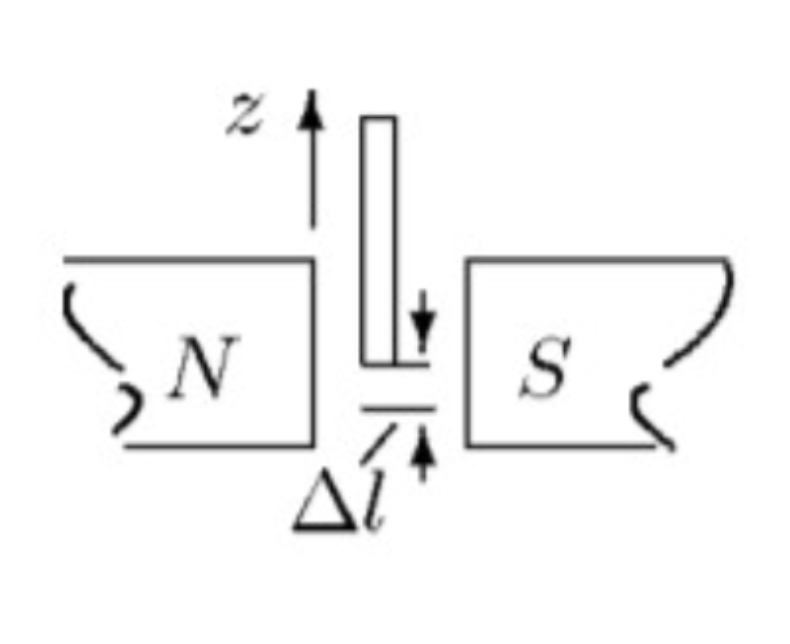
\includegraphics[width=4cm]{Screenshot_2.jpg}
    \caption{Расположение образца в зазоре электромагнита}
    \label{pic:1}
\end{wrapfigure}

Воспользуемся для расчёта энергетическими соображениями. Магнитная сила может быть вычислена как производная от магнитной энергии по перемещению. Из теории известно, что эту производную следует брать со знаком минус, когда образец находится в поле постоянного магнита, или со знаком плюс, как в нашем случае, когда поле в зазоре создаётся электромагнитом, ток $ I $ в обмотках которого поддерживается постоянным.

При смещении образца на расстояние $ \Delta l $ вниз магнитная сила, действующая на него, равна

\begin{equation}\label{1}
F = \left(\frac{\Delta W_m}{\Delta l}\right)_I,
\end{equation}
где $ \Delta W_m $ -- изменение магнитной энергии системы при постоянном токе
в обмотке электромагнита и, следовательно, при постоянной величине
магнитного поля в зазоре.

Магнитная энергия рассчитывается по формуле

\begin{equation}\label{2}
W_m=\frac{1}{2}\int HBd\,V = \frac{1}{2\mu_0}\int\frac{B^2}{\mu}d\,V,
\end{equation}
где интеграл распространён на всё пространство. При смещении образца магнитная энергия меняется только в области зазора (в объёме площади $ s $ и высоты $ \Delta l $), а около верхнего конца стержня остаётся неизменной, поскольку магнитного поля там практически нет. Принимая поле внутри стержня равным измеренному нами полю в зазоре $ B $, получим

\begin{equation}\label{3}
\Delta W_m=\frac{1}{2\mu_0}\frac{B^2}{\mu}s\Delta l - \frac{1}{2\mu_0}B^2 s\Delta l = -\frac{\chi}{2\mu_0\mu}B^2s\Delta l.
\end{equation}

Следовательно, на образец действует сила
\begin{equation}\label{4}
F = -\frac{\chi}{2\mu_0\mu}B^2s.
\end{equation}

Знак силы, действующей на образец, зависит от знака $ \chi $: образцы из парамагнитных материалов $( \chi  > 0)$ втягиваются в зазор электромагнита, а диамагнитные образцы $ (\chi < 0) $ выталкиваются из него.

Пренебрегая отличием $ \mu $ от единицы, получаем окончательно расчётную формулу в виде

\begin{equation}\label{5}
F = -\frac{\chi B^2s}{2\mu_0}.
\end{equation}

Измерив силу, действующую на образец в магнитном поле $ B $, можно рассчитать магнитную восприимчивость образца.


\section{Экспериментальная установка}

\begin{wrapfigure}{r}{6.5cm}
    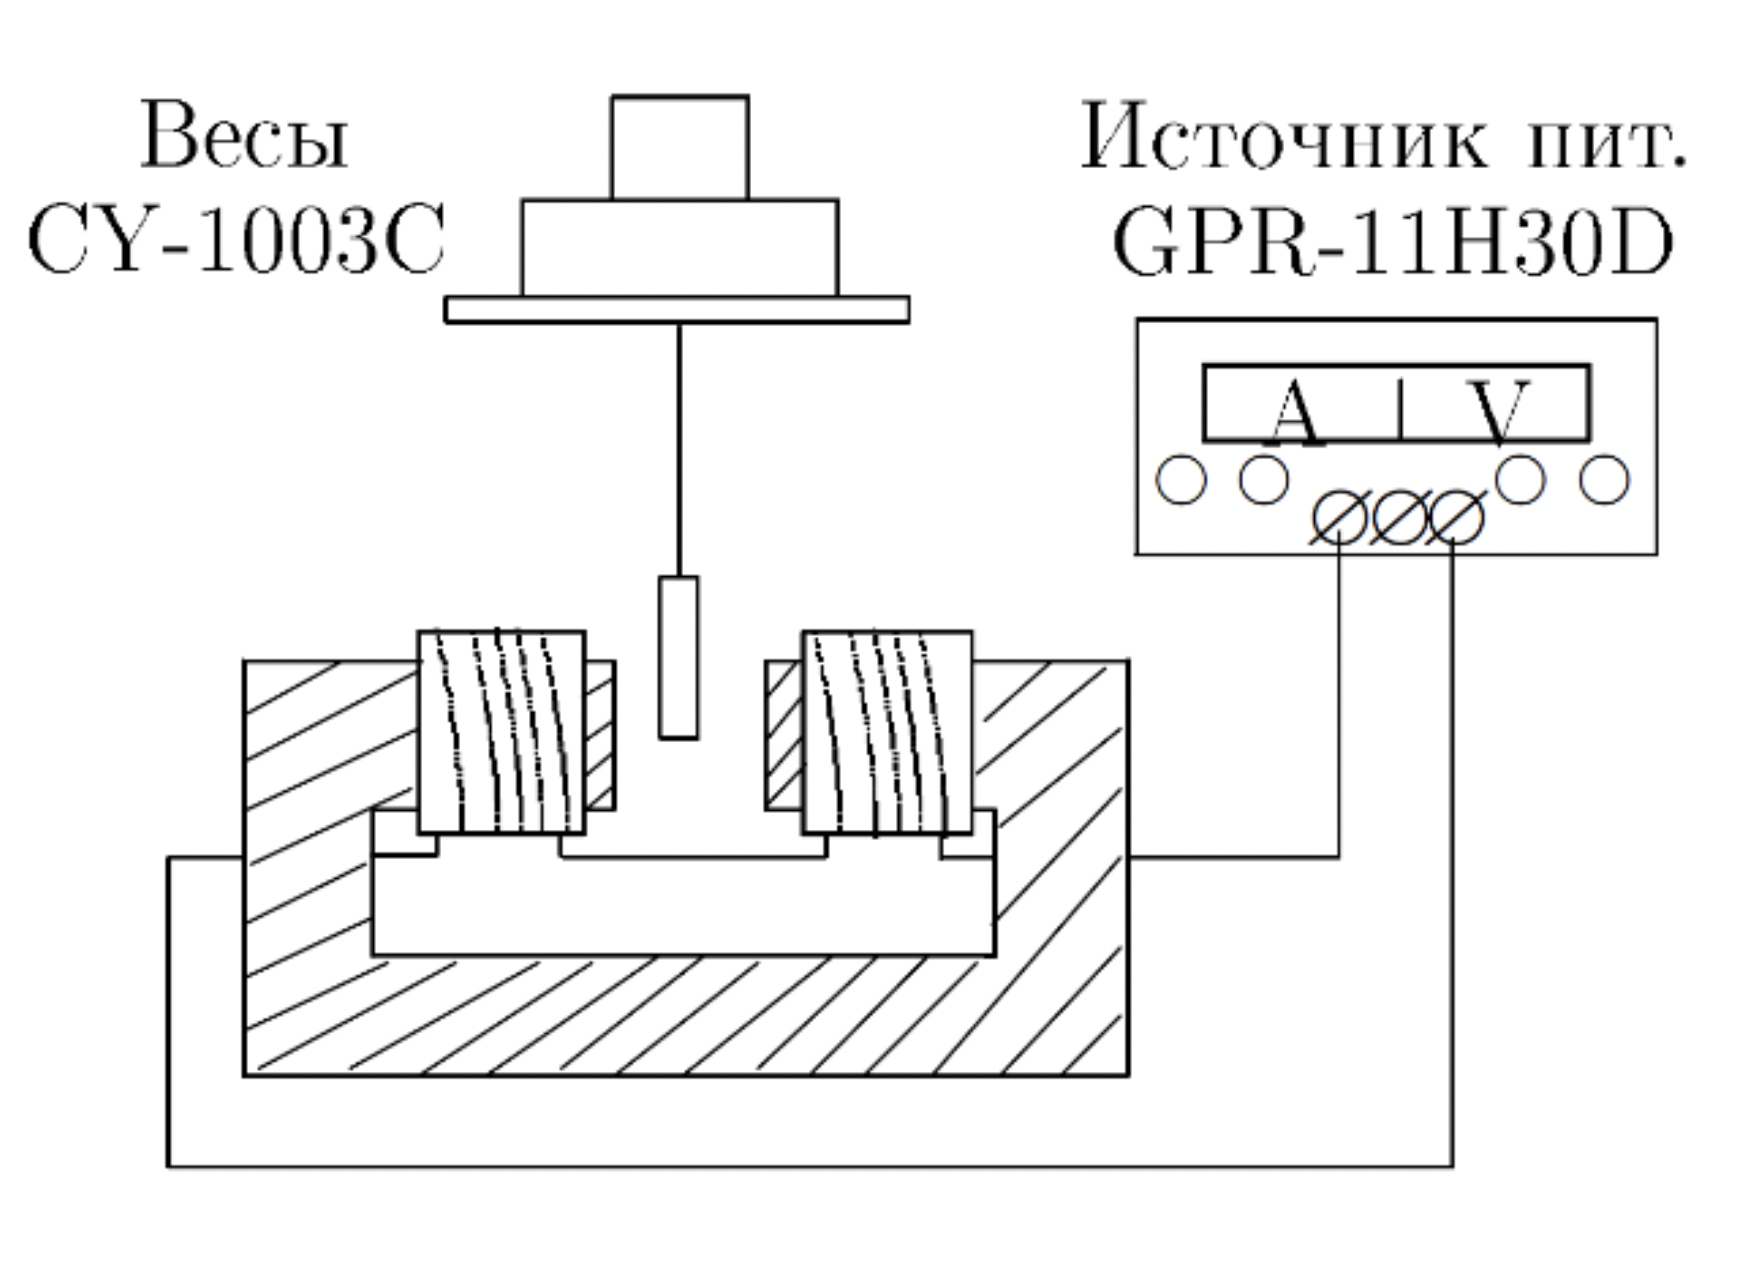
\includegraphics[width=6.5cm]{Screenshot_1.png}
    \caption{Схема экспериментальной установки.}
    \label{pic:2}
\end{wrapfigure}


Магнитное поле с максимальной индукцией $ \simeq 1 $ Т создаётся в зазоре электромагнита, питаемого постоянным током. Диаметр полюсов существенно превосходит ширину зазора, поэтому поле в средней части зазора достаточно однородно. Величина тока, проходящего через обмотки электромагнита, задаётся регулируемым источником питания GPR и измеряется амперметром $ А $, встроенным в источник питания. Градуировка электромагнита (связь между индукцией магнитного поля $ B $ в зазоре электромагнита и силой тока $ I $ в его обмотках) производится при помощи милливеберметра.


При измерениях образцы поочерёдно подвешиваются к весам так, что один конец образца оказывается в зазоре электромагнита, а другой -- вне зазора, где индукцией магнитного поля можно пренебречь. При помощи весов определяется перегрузка $ \Delta P = F $ -- сила, действующая на образец со стороны магнитного поля.


Силы, действующие на диа- и парамагнитные образцы, очень малы. Небольшие примеси ферромагнетиков (сотые доли процента железа или никеля) способны кардинально изменить результат опыта, поэтому образцы были специально отобраны.







\section{Ход работы:}

1. Максимальное значение изменения тока через обмотки: $I_{max}=3,02A$.

2. Прокалибруем электромагнит для этого снимем зависимость магнитной индукции от силы тока с помощью тесламетра:

\begin{table}[!ht]
    \centering
    \begin{tabular}{|l|l|l|l|l|l|l|l|l|l|}
    \hline
        I, А & 0,3 & 0,6 & 0,91 & 1,2 & 1,5 & 1,81 & 2,2 & 2,6 & 3,02 \\ \hline
        В, мТл & 99 & 185,3 & 288,6 & 372,5 & 463 & 545 & 653,7 & 735,2 & 806,9 \\ \hline
    \end{tabular}
\end{table}


По этим данным построим график:

\begin{figure}[H]
\center{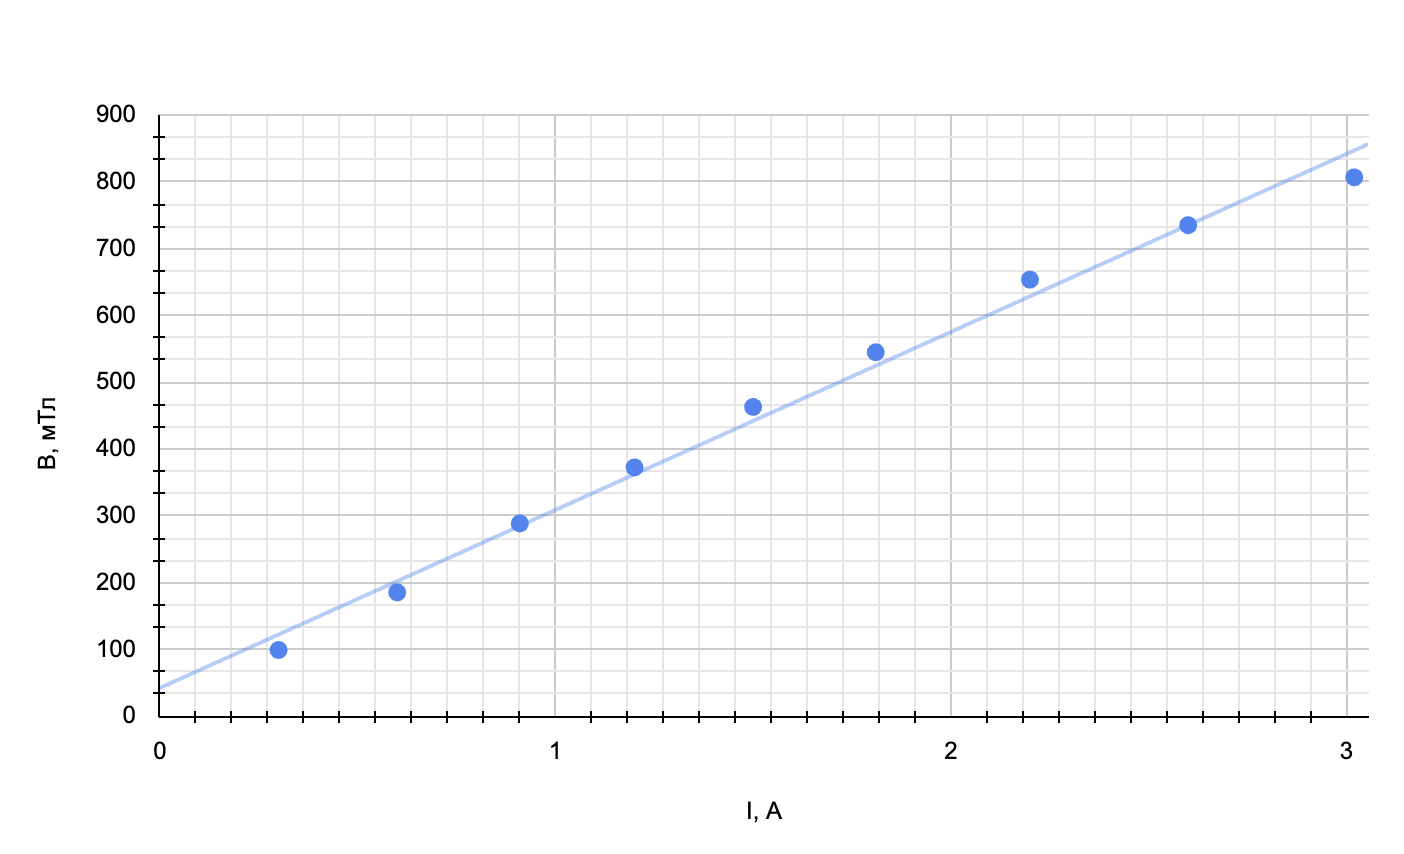
\includegraphics[scale=0.7]{Screen_3.png}}
\caption{График зависимости магнитной индукции В от силы тока I. Градуировочная кривая.}
\label{pic:3}
\end{figure}

Апроксимируем по МНК, получаем зависимость вида $y = bx - a$, где коэффициенты:

\[b = 267 \pm 8 \frac{мТл}{А}\]
\[а = 42 \pm 7 мТл\]

\newpage

3. \textbf{Измереним силы, действующие на образцы в магнитном поле}

\medskip

При нулевом токе через электромагнит подвесим к весам один из образцов так, чтобы он не касался наконечников электромагнита. Обнулим показания весов, чтобы измерять непосредственно перегрузки $ \Delta P = F $ -- силы, действующей на образец при различных токах в обмотках электромагнита.

Установим минимальное из выбранных при калибровке магнита значение тока $ A_{min} $ и проведём измерение перегрузки. Повторим измерения $ \Delta P = f(I) $ для значений тока в диапазоне от $ A_{min} $ до $ A_{max} $. Проведём такие измерения для различных образцов. Результаты измерений занесём в таблицу:

\begin{table}[!ht]
\centering
\begin{tabular}{|c|cccc|}
\hline
\multicolumn{1}{|l|}{\textbf{}} & \multicolumn{1}{c|}{\cellcolor[HTML]{FFFFFF}Cu} & \multicolumn{1}{c|}{\cellcolor[HTML]{FFFFFF}Al} & \multicolumn{1}{c|}{\cellcolor[HTML]{FFFFFF}Gr} & \cellcolor[HTML]{FFFFFF}Wr \\ \hline
\textbf{I, А} & \multicolumn{4}{c|}{\cellcolor[HTML]{FFFFFF} Показания весов, г} \\ \hline
0,3 & \multicolumn{1}{c|}{-0,001} & \multicolumn{1}{c|}{0} & \multicolumn{1}{c|}{0,007} & 0 \\ \hline
0,6 & \multicolumn{1}{c|}{-0,002} & \multicolumn{1}{c|}{0,001} & \multicolumn{1}{c|}{0,017} & 0 \\ \hline
0,91 & \multicolumn{1}{c|}{-0,004} & \multicolumn{1}{c|}{0,004} & \multicolumn{1}{c|}{0,025} & 0 \\ \hline
1,2 & \multicolumn{1}{c|}{-0,006} & \multicolumn{1}{c|}{0,009} & \multicolumn{1}{c|}{0,029} & 0 \\ \hline
1,5 & \multicolumn{1}{c|}{-0,008} & \multicolumn{1}{c|}{0,014} & \multicolumn{1}{c|}{0,03} & 0 \\ \hline
1,81 & \multicolumn{1}{c|}{-0,011} & \multicolumn{1}{c|}{0,019} & \multicolumn{1}{c|}{0,027} & 0 \\ \hline
2,2 & \multicolumn{1}{c|}{-0,015} & \multicolumn{1}{c|}{0,028} & \multicolumn{1}{c|}{0,016} & 0 \\ \hline
2,6 & \multicolumn{1}{c|}{-0,019} & \multicolumn{1}{c|}{0,036} & \multicolumn{1}{c|}{0} & 0 \\ \hline
3,02 & \multicolumn{1}{c|}{-0,024} & \multicolumn{1}{c|}{0,046} & \multicolumn{1}{c|}{-0,021} & 0 \\ \hline
\end{tabular}
\end{table}

4. Для построения графиков зависимостей $ |\Delta P| = f(B^2) $ переведём $ I $ в $ B $ по градуировочным данным согласно таблице градуировки и домножим на $g$, чтобы получить $\Delta P$. Данные, полученные после обработки занесём в таблицу:

\begin{table}[!ht]
\centering
\begin{tabular}{|c|cccc|}
\hline
\multicolumn{1}{|l|}{\textbf{}} & \multicolumn{1}{c|}{\cellcolor[HTML]{FFFFFF}Cu} & \multicolumn{1}{c|}{\cellcolor[HTML]{FFFFFF}Al} & \multicolumn{1}{c|}{\cellcolor[HTML]{FFFFFF}Gr} & \multicolumn{1}{c|}{\cellcolor[HTML]{FFFFFF}Wr} \\ \hline
\textbf{$В^2, Тл^2$} & \multicolumn{4}{c|}{\cellcolor[HTML]{FFFFFF}Перегрузки $\Delta P, мкH$} \\ \hline
0,010 & \multicolumn{1}{r|}{-0,010} & \multicolumn{1}{r|}{0,000} & \multicolumn{1}{r|}{0,069} & 0,000 \\ \hline
0,034 & \multicolumn{1}{r|}{-0,020} & \multicolumn{1}{r|}{0,010} & \multicolumn{1}{r|}{0,167} & 0,000 \\ \hline
0,083 & \multicolumn{1}{r|}{-0,039} & \multicolumn{1}{r|}{0,039} & \multicolumn{1}{r|}{0,245} & 0,000 \\ \hline
0,139 & \multicolumn{1}{r|}{-0,059} & \multicolumn{1}{r|}{0,088} & \multicolumn{1}{r|}{0,284} & 0,000 \\ \hline
0,214 & \multicolumn{1}{r|}{-0,078} & \multicolumn{1}{r|}{0,137} & \multicolumn{1}{r|}{0,294} & 0,000 \\ \hline
0,297 & \multicolumn{1}{r|}{-0,108} & \multicolumn{1}{r|}{0,186} & \multicolumn{1}{r|}{0,265} & 0,000 \\ \hline
0,427 & \multicolumn{1}{r|}{-0,147} & \multicolumn{1}{r|}{0,274} & \multicolumn{1}{r|}{0,157} & 0,000 \\ \hline
0,541 & \multicolumn{1}{r|}{-0,186} & \multicolumn{1}{r|}{0,353} & \multicolumn{1}{r|}{0,000} & 0,000 \\ \hline
0,651 & \multicolumn{1}{r|}{-0,235} & \multicolumn{1}{r|}{0,451} & \multicolumn{1}{r|}{-0,206} & 0,000 \\ \hline
\end{tabular}
\end{table}


Построим графики:

\begin{figure}[H]
\center{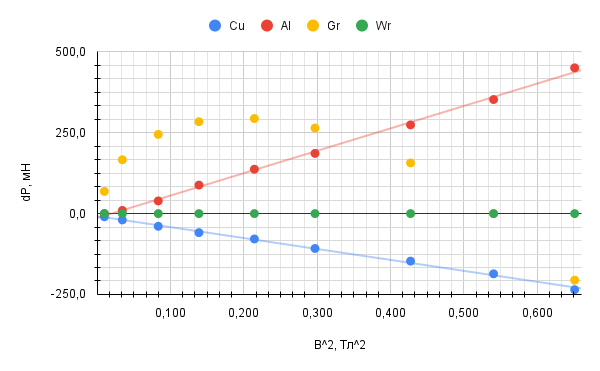
\includegraphics[scale=0.8]{chart.png}}
\caption{Графики $ |\Delta P| = f(B^2) $ для разных материалов}
\label{pic:3}
\end{figure}

Апроксимируем к уравнению $y = bx$:

\[Cu: b = (-342 \pm 6) \frac{мкН}{Тл^2}\]

\[Al: b = (686 \pm 10) \frac{мкН}{Тл^2}\]

\[Wr: b = (0 \pm 0) \frac{мкН}{Тл^2}\]

5. Воспользуемся формулой:

\begin{equation*}\label{5}
F = -\frac{\chi B^2s}{2\mu_0}.
\end{equation*}

\begin{equation}\label{6}
b = \frac{\chi s}{2\mu_0}.
\end{equation}

Отсюда
\begin{equation}\label{7}
\boxed{\chi = \frac{2\mu_0 b}{s}}
\end{equation}

Учитывая, что:
$ s = (0,78 \pm 0,02) cм^2$ для образцов алюминия, меди и графита. Магнитная постоянная $\mu_0 = 4 \pi \cdot 10^{-7} \frac{H}{A^2}$ Вычисляем $\chi$:

\[\chi_{Cu} = (-1,1 \pm 0,1)\cdot 10^{-5} \]

\[\chi_{Al} = (2,2 \pm 0,1)\cdot 10^{-5} \]

\[\chi_{Wr} = 0\]

Замечание: 

1) Графит проявил себя неоднозначно, его поведение похоже на квадратичную зависимость: ближе к нулю он проявляет парамагнетичские свойства, а далее ведет себя, как диамагнетик, чем в теории и является.

2) Пронаблюдать парамагнетические свойства вольфрама не удалось, скорее всего из-за того, что образец был слишком короток и в достаточной степени не доставал до магнита.

\section{Вывод} 

В ходе лабараторной работы была измерена магнитная восприимчивость диа- и пара- магнетиков. Были исследованы образцы алюминия, меди, графита и вольфрама. Для алюминия и меди табличные значения магнитной восприимчивости равны \underline{$ \chi_{Cu}^t = -1,0 \cdot 10^{-5} $} и \underline{$ \chi_{Al}^t = 2,3 \cdot 10^{-5} $} соответственно. Полученные значения:  \underline {$\chi_{Cu} = (-1,1 \pm 0,1)\cdot 10^{-5}$}, \underline{$\chi_{Al} = (2,2 \pm 0,1)\cdot 10^{-5}$}. Экспериментальные данные совпадают с табличными в пределах погрешностей. Исходя из этого можно сказать, что алюминий является парамагнетиком $ (\chi > 0) $, а медь в свою очередь -- диамагнетиком $ (\chi < 0) $.

Таким образом, данный метод измерения магнитной проницаемости материалов является рабочим и позволяет с хорошей точность определить эту величину для различных исследуемых образцов.


Результаты эксперимента для графита не столь однозначны. Несмотря на то, что графит должен демонстрировать диамагнетизм, в нашем опыте на некоторой области он проявил себя иначе. 

Пронаблюдать парамагнетические свойства вольфрама не удалось.


\end{document}